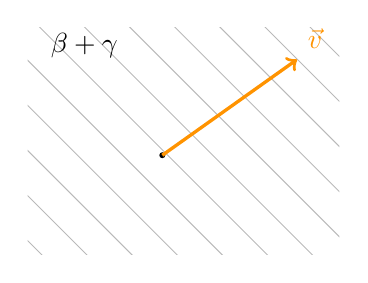
\begin{tikzpicture}[scale=0.9]
  % beta + gamma: diagonal family of lines
  \clip (-2.2,-1.6) rectangle (2.2,1.6);
  \begin{scope}[rotate=45]
    \foreach \x in {-3,-2.55,...,3} {
      \draw[gray!55, line width=0.35pt] (\x,-3) -- (\x,3);
    }
  \end{scope}

  % vector v
  \fill[black] (-0.3,-0.2) circle (1.2pt);
  \draw[->, very thick, orange!85!yellow] (-0.3,-0.2) -- (1.6,1.15) node[above right] {$\vec{v}$};

  \node at (-1.4,1.35) {$\beta + \gamma$};
\end{tikzpicture}
